\documentclass[twoside]{book}

% Packages required by doxygen
\usepackage{fixltx2e}
\usepackage{calc}
\usepackage{doxygen}
\usepackage[export]{adjustbox} % also loads graphicx
\usepackage{graphicx}
\usepackage[utf8]{inputenc}
\usepackage{makeidx}
\usepackage{multicol}
\usepackage{multirow}
\PassOptionsToPackage{warn}{textcomp}
\usepackage{textcomp}
\usepackage[nointegrals]{wasysym}
\usepackage[table]{xcolor}

% Font selection
\usepackage[T1]{fontenc}
\usepackage[scaled=.90]{helvet}
\usepackage{courier}
\usepackage{amssymb}
\usepackage{sectsty}
\renewcommand{\familydefault}{\sfdefault}
\allsectionsfont{%
  \fontseries{bc}\selectfont%
  \color{darkgray}%
}
\renewcommand{\DoxyLabelFont}{%
  \fontseries{bc}\selectfont%
  \color{darkgray}%
}
\newcommand{\+}{\discretionary{\mbox{\scriptsize$\hookleftarrow$}}{}{}}

% Page & text layout
\usepackage{geometry}
\geometry{%
  a4paper,%
  top=2.5cm,%
  bottom=2.5cm,%
  left=2.5cm,%
  right=2.5cm%
}
\tolerance=750
\hfuzz=15pt
\hbadness=750
\setlength{\emergencystretch}{15pt}
\setlength{\parindent}{0cm}
\setlength{\parskip}{3ex plus 2ex minus 2ex}
\makeatletter
\renewcommand{\paragraph}{%
  \@startsection{paragraph}{4}{0ex}{-1.0ex}{1.0ex}{%
    \normalfont\normalsize\bfseries\SS@parafont%
  }%
}
\renewcommand{\subparagraph}{%
  \@startsection{subparagraph}{5}{0ex}{-1.0ex}{1.0ex}{%
    \normalfont\normalsize\bfseries\SS@subparafont%
  }%
}
\makeatother

% Headers & footers
\usepackage{fancyhdr}
\pagestyle{fancyplain}
\fancyhead[LE]{\fancyplain{}{\bfseries\thepage}}
\fancyhead[CE]{\fancyplain{}{}}
\fancyhead[RE]{\fancyplain{}{\bfseries\leftmark}}
\fancyhead[LO]{\fancyplain{}{\bfseries\rightmark}}
\fancyhead[CO]{\fancyplain{}{}}
\fancyhead[RO]{\fancyplain{}{\bfseries\thepage}}
\fancyfoot[LE]{\fancyplain{}{}}
\fancyfoot[CE]{\fancyplain{}{}}
\fancyfoot[RE]{\fancyplain{}{\bfseries\scriptsize Generated by Doxygen }}
\fancyfoot[LO]{\fancyplain{}{\bfseries\scriptsize Generated by Doxygen }}
\fancyfoot[CO]{\fancyplain{}{}}
\fancyfoot[RO]{\fancyplain{}{}}
\renewcommand{\footrulewidth}{0.4pt}
\renewcommand{\chaptermark}[1]{%
  \markboth{#1}{}%
}
\renewcommand{\sectionmark}[1]{%
  \markright{\thesection\ #1}%
}

% Indices & bibliography
\usepackage{natbib}
\usepackage[titles]{tocloft}
\setcounter{tocdepth}{3}
\setcounter{secnumdepth}{5}
\makeindex

% Hyperlinks (required, but should be loaded last)
\usepackage{ifpdf}
\ifpdf
  \usepackage[pdftex,pagebackref=true]{hyperref}
\else
  \usepackage[ps2pdf,pagebackref=true]{hyperref}
\fi
\hypersetup{%
  colorlinks=true,%
  linkcolor=blue,%
  citecolor=blue,%
  unicode%
}

% Custom commands
\newcommand{\clearemptydoublepage}{%
  \newpage{\pagestyle{empty}\cleardoublepage}%
}

\usepackage{caption}
\captionsetup{labelsep=space,justification=centering,font={bf},singlelinecheck=off,skip=4pt,position=top}

%===== C O N T E N T S =====

\begin{document}

% Titlepage & ToC
\hypersetup{pageanchor=false,
             bookmarksnumbered=true,
             pdfencoding=unicode
            }
\pagenumbering{alph}
\begin{titlepage}
\vspace*{7cm}
\begin{center}%
{\Large Jeu\+\_\+de\+\_\+la\+\_\+vie }\\
\vspace*{1cm}
{\large Generated by Doxygen 1.8.13}\\
\end{center}
\end{titlepage}
\clearemptydoublepage
\pagenumbering{roman}
\tableofcontents
\clearemptydoublepage
\pagenumbering{arabic}
\hypersetup{pageanchor=true}

%--- Begin generated contents ---
\chapter{Data Structure Index}
\section{Data Structures}
Here are the data structures with brief descriptions\+:\begin{DoxyCompactList}
\item\contentsline{section}{\hyperlink{structgrille}{grille} }{\pageref{structgrille}}{}
\end{DoxyCompactList}

\chapter{File Index}
\section{File List}
Here is a list of all documented files with brief descriptions\+:\begin{DoxyCompactList}
\item\contentsline{section}{include/\hyperlink{grille_8h}{grille.\+h} }{\pageref{grille_8h}}{}
\item\contentsline{section}{include/\hyperlink{io_8h}{io.\+h} }{\pageref{io_8h}}{}
\item\contentsline{section}{include/\hyperlink{jeu_8h}{jeu.\+h} }{\pageref{jeu_8h}}{}
\item\contentsline{section}{src/\hyperlink{grille_8c}{grille.\+c} }{\pageref{grille_8c}}{}
\item\contentsline{section}{src/\hyperlink{io_8c}{io.\+c} }{\pageref{io_8c}}{}
\item\contentsline{section}{src/\hyperlink{jeu_8c}{jeu.\+c} }{\pageref{jeu_8c}}{}
\end{DoxyCompactList}

\chapter{Data Structure Documentation}
\hypertarget{structgrille}{}\section{grille Struct Reference}
\label{structgrille}\index{grille@{grille}}
\subsection*{Data Fields}
\begin{DoxyCompactItemize}
\item 
\mbox{\Hypertarget{structgrille_a0b4da1e205825df205b0c004d105d62a}\label{structgrille_a0b4da1e205825df205b0c004d105d62a}} 
int {\bfseries nbl}
\item 
\mbox{\Hypertarget{structgrille_a48d6706d41bee6fff9200d872b8b0cd0}\label{structgrille_a48d6706d41bee6fff9200d872b8b0cd0}} 
int {\bfseries nbc}
\item 
\mbox{\Hypertarget{structgrille_a428cf0c0297ce04e0206ba0067ac3b42}\label{structgrille_a428cf0c0297ce04e0206ba0067ac3b42}} 
int $\ast$$\ast$ {\bfseries cellules}
\end{DoxyCompactItemize}


The documentation for this struct was generated from the following file\+:\begin{DoxyCompactItemize}
\item 
include/\hyperlink{grille_8h}{grille.\+h}\end{DoxyCompactItemize}

\chapter{File Documentation}
\hypertarget{grille_8h}{}\section{include/grille.h File Reference}
\label{grille_8h}\index{include/grille.\+h@{include/grille.\+h}}
{\ttfamily \#include $<$stdlib.\+h$>$}\newline
{\ttfamily \#include $<$stdio.\+h$>$}\newline
{\ttfamily \#include $<$assert.\+h$>$}\newline
Include dependency graph for grille.\+h\+:\nopagebreak
\begin{figure}[H]
\begin{center}
\leavevmode
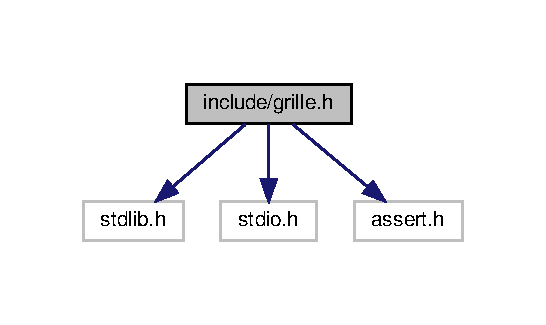
\includegraphics[width=262pt]{grille_8h__incl}
\end{center}
\end{figure}
This graph shows which files directly or indirectly include this file\+:\nopagebreak
\begin{figure}[H]
\begin{center}
\leavevmode
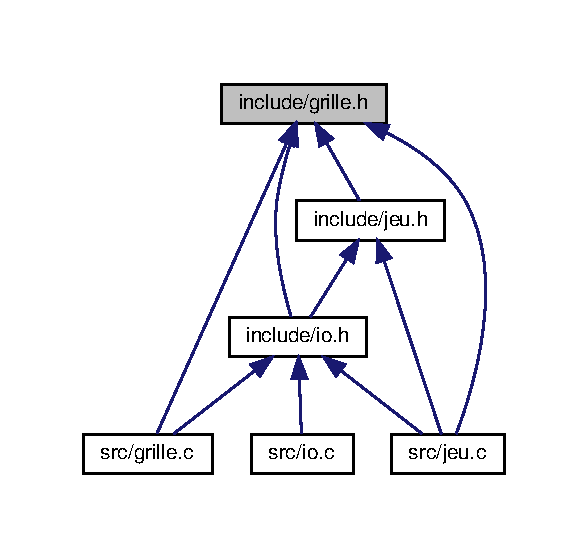
\includegraphics[width=282pt]{grille_8h__dep__incl}
\end{center}
\end{figure}
\subsection*{Data Structures}
\begin{DoxyCompactItemize}
\item 
struct \hyperlink{structgrille}{grille}
\end{DoxyCompactItemize}
\subsection*{Functions}
\begin{DoxyCompactItemize}
\item 
void \hyperlink{grille_8h_ae621f51c60aa4fafaa0c9f6c9b5a4036}{alloue\+\_\+grille} (int l, int c, \hyperlink{structgrille}{grille} $\ast$g)
\item 
void \hyperlink{grille_8h_a7074b2b15576e9d2b3cd15c3a1dc7012}{libere\+\_\+grille} (\hyperlink{structgrille}{grille} $\ast$g)
\item 
void \hyperlink{grille_8h_adf5501cc0bbad28f5ffc561d92197e4e}{init\+\_\+grille\+\_\+from\+\_\+file} (char $\ast$filename, \hyperlink{structgrille}{grille} $\ast$g)
\item 
void \hyperlink{grille_8h_a63b3ae16c86b568f6aa8f9ce84128b1e}{copie\+\_\+grille} (\hyperlink{structgrille}{grille} gs, \hyperlink{structgrille}{grille} gd)
\end{DoxyCompactItemize}
\subsection*{Variables}
\begin{DoxyCompactItemize}
\item 
\mbox{\Hypertarget{grille_8h_a852233e3ec97f7c44944c67998337e26}\label{grille_8h_a852233e3ec97f7c44944c67998337e26}} 
int {\bfseries vieillissement}
\end{DoxyCompactItemize}


\subsection{Detailed Description}
header pour les fonctions sur les grilles \begin{DoxyAuthor}{Author}
Maxime M\+A\+I\+RE 
\end{DoxyAuthor}


\subsection{Function Documentation}
\mbox{\Hypertarget{grille_8h_ae621f51c60aa4fafaa0c9f6c9b5a4036}\label{grille_8h_ae621f51c60aa4fafaa0c9f6c9b5a4036}} 
\index{grille.\+h@{grille.\+h}!alloue\+\_\+grille@{alloue\+\_\+grille}}
\index{alloue\+\_\+grille@{alloue\+\_\+grille}!grille.\+h@{grille.\+h}}
\subsubsection{\texorpdfstring{alloue\+\_\+grille()}{alloue\_grille()}}
{\footnotesize\ttfamily void alloue\+\_\+grille (\begin{DoxyParamCaption}\item[{int}]{l,  }\item[{int}]{c,  }\item[{\hyperlink{structgrille}{grille} $\ast$}]{g }\end{DoxyParamCaption})}


\begin{DoxyParams}{Parameters}
{\em l} & est un entier representant le nombre de ligne a alloue pour la grille g \\
\hline
{\em c} & est un entier representant le nombre de colonne a alloue pour la grille g \\
\hline
{\em $\ast$g} & est un pointeur sur une grille \\
\hline
\end{DoxyParams}
\begin{DoxyReturn}{Returns}
Retourne vide, mais alloue une grille de ligne l et de colonne c 
\end{DoxyReturn}
\mbox{\Hypertarget{grille_8h_a63b3ae16c86b568f6aa8f9ce84128b1e}\label{grille_8h_a63b3ae16c86b568f6aa8f9ce84128b1e}} 
\index{grille.\+h@{grille.\+h}!copie\+\_\+grille@{copie\+\_\+grille}}
\index{copie\+\_\+grille@{copie\+\_\+grille}!grille.\+h@{grille.\+h}}
\subsubsection{\texorpdfstring{copie\+\_\+grille()}{copie\_grille()}}
{\footnotesize\ttfamily void copie\+\_\+grille (\begin{DoxyParamCaption}\item[{\hyperlink{structgrille}{grille}}]{gs,  }\item[{\hyperlink{structgrille}{grille}}]{gd }\end{DoxyParamCaption})}


\begin{DoxyParams}{Parameters}
{\em gs} & est une grille \\
\hline
{\em gd} & est une grille \\
\hline
\end{DoxyParams}
\begin{DoxyReturn}{Returns}
Retourne vide, mais recopie la grille gs dans la grille gd 
\end{DoxyReturn}
\mbox{\Hypertarget{grille_8h_adf5501cc0bbad28f5ffc561d92197e4e}\label{grille_8h_adf5501cc0bbad28f5ffc561d92197e4e}} 
\index{grille.\+h@{grille.\+h}!init\+\_\+grille\+\_\+from\+\_\+file@{init\+\_\+grille\+\_\+from\+\_\+file}}
\index{init\+\_\+grille\+\_\+from\+\_\+file@{init\+\_\+grille\+\_\+from\+\_\+file}!grille.\+h@{grille.\+h}}
\subsubsection{\texorpdfstring{init\+\_\+grille\+\_\+from\+\_\+file()}{init\_grille\_from\_file()}}
{\footnotesize\ttfamily void init\+\_\+grille\+\_\+from\+\_\+file (\begin{DoxyParamCaption}\item[{char $\ast$}]{filename,  }\item[{\hyperlink{structgrille}{grille} $\ast$}]{g }\end{DoxyParamCaption})}


\begin{DoxyParams}{Parameters}
{\em $\ast$filename} & est un tableau de charactere permettant de chercher un fichier a scanf \\
\hline
{\em $\ast$g} & est un pointeur sur une grille \\
\hline
\end{DoxyParams}
\begin{DoxyReturn}{Returns}
Retourne vide, mais alloue et initalise la grille g à partir d\textquotesingle{}un fichier 
\end{DoxyReturn}
\mbox{\Hypertarget{grille_8h_a7074b2b15576e9d2b3cd15c3a1dc7012}\label{grille_8h_a7074b2b15576e9d2b3cd15c3a1dc7012}} 
\index{grille.\+h@{grille.\+h}!libere\+\_\+grille@{libere\+\_\+grille}}
\index{libere\+\_\+grille@{libere\+\_\+grille}!grille.\+h@{grille.\+h}}
\subsubsection{\texorpdfstring{libere\+\_\+grille()}{libere\_grille()}}
{\footnotesize\ttfamily void libere\+\_\+grille (\begin{DoxyParamCaption}\item[{\hyperlink{structgrille}{grille} $\ast$}]{g }\end{DoxyParamCaption})}


\begin{DoxyParams}{Parameters}
{\em $\ast$g} & est un pointeur sur une grille \\
\hline
\end{DoxyParams}
\begin{DoxyReturn}{Returns}
Retourne vide, mais libere la grille g 
\end{DoxyReturn}

\hypertarget{io_8h}{}\section{include/io.h File Reference}
\label{io_8h}\index{include/io.\+h@{include/io.\+h}}
{\ttfamily \#include $<$stdio.\+h$>$}\newline
{\ttfamily \#include \char`\"{}grille.\+h\char`\"{}}\newline
{\ttfamily \#include \char`\"{}jeu.\+h\char`\"{}}\newline
Include dependency graph for io.\+h\+:
\nopagebreak
\begin{figure}[H]
\begin{center}
\leavevmode
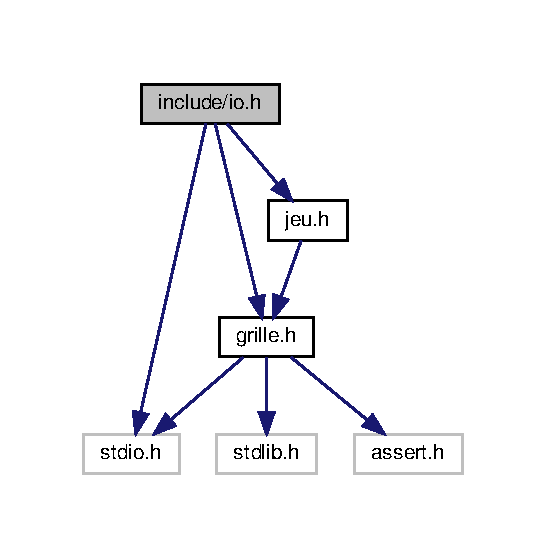
\includegraphics[width=262pt]{io_8h__incl}
\end{center}
\end{figure}
This graph shows which files directly or indirectly include this file\+:
\nopagebreak
\begin{figure}[H]
\begin{center}
\leavevmode
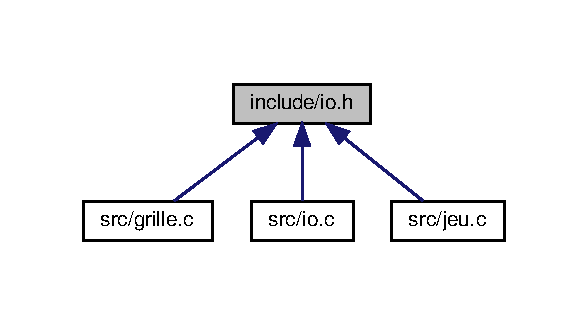
\includegraphics[width=282pt]{io_8h__dep__incl}
\end{center}
\end{figure}
\subsection*{Functions}
\begin{DoxyCompactItemize}
\item 
void \hyperlink{io_8h_a634cf584c380ce221d5d4199f3e813bd}{affiche\+\_\+trait} (int c)
\item 
void \hyperlink{io_8h_a3f3ff78e56fcf21a932ff73b70635554}{affiche\+\_\+ligne} (int c, int $\ast$ligne)
\item 
void \hyperlink{io_8h_a90cb8ec05374b46d9995705ed4954f34}{affiche\+\_\+grille} (\hyperlink{structgrille}{grille} g)
\item 
void \hyperlink{io_8h_ab36a6f8957cd3e682119007836ce6ad5}{efface\+\_\+grille} (\hyperlink{structgrille}{grille} g)
\item 
void \hyperlink{io_8h_a88493b3c55828670e47150a95ed7db5b}{debut\+\_\+jeu} (\hyperlink{structgrille}{grille} $\ast$g, \hyperlink{structgrille}{grille} $\ast$gc)
\end{DoxyCompactItemize}


\subsection{Detailed Description}
header pour les fonctions d\textquotesingle{}affichage \begin{DoxyAuthor}{Author}
Maxime M\+A\+I\+RE 
\end{DoxyAuthor}


\subsection{Function Documentation}
\mbox{\Hypertarget{io_8h_a90cb8ec05374b46d9995705ed4954f34}\label{io_8h_a90cb8ec05374b46d9995705ed4954f34}} 
\index{io.\+h@{io.\+h}!affiche\+\_\+grille@{affiche\+\_\+grille}}
\index{affiche\+\_\+grille@{affiche\+\_\+grille}!io.\+h@{io.\+h}}
\subsubsection{\texorpdfstring{affiche\+\_\+grille()}{affiche\_grille()}}
{\footnotesize\ttfamily void affiche\+\_\+grille (\begin{DoxyParamCaption}\item[{\hyperlink{structgrille}{grille}}]{g }\end{DoxyParamCaption})}


\begin{DoxyParams}{Parameters}
{\em g} & est une grille \\
\hline
\end{DoxyParams}
\begin{DoxyReturn}{Returns}
Retourne vide, mais affiche la grille g 
\end{DoxyReturn}
\mbox{\Hypertarget{io_8h_a3f3ff78e56fcf21a932ff73b70635554}\label{io_8h_a3f3ff78e56fcf21a932ff73b70635554}} 
\index{io.\+h@{io.\+h}!affiche\+\_\+ligne@{affiche\+\_\+ligne}}
\index{affiche\+\_\+ligne@{affiche\+\_\+ligne}!io.\+h@{io.\+h}}
\subsubsection{\texorpdfstring{affiche\+\_\+ligne()}{affiche\_ligne()}}
{\footnotesize\ttfamily void affiche\+\_\+ligne (\begin{DoxyParamCaption}\item[{int}]{c,  }\item[{int $\ast$}]{ligne }\end{DoxyParamCaption})}


\begin{DoxyParams}{Parameters}
{\em c} & est le nombre de colonne a affiché \\
\hline
{\em ligne} & est un pointeur sur entier \\
\hline
\end{DoxyParams}
\begin{DoxyReturn}{Returns}
Retourne vide, mais affiche des caracteres 
\end{DoxyReturn}
\mbox{\Hypertarget{io_8h_a634cf584c380ce221d5d4199f3e813bd}\label{io_8h_a634cf584c380ce221d5d4199f3e813bd}} 
\index{io.\+h@{io.\+h}!affiche\+\_\+trait@{affiche\+\_\+trait}}
\index{affiche\+\_\+trait@{affiche\+\_\+trait}!io.\+h@{io.\+h}}
\subsubsection{\texorpdfstring{affiche\+\_\+trait()}{affiche\_trait()}}
{\footnotesize\ttfamily void affiche\+\_\+trait (\begin{DoxyParamCaption}\item[{int}]{c }\end{DoxyParamCaption})}


\begin{DoxyParams}{Parameters}
{\em c} & est le nombre de colonne a affiché \\
\hline
\end{DoxyParams}
\begin{DoxyReturn}{Returns}
Retourne vide, mais affiche des caracteres 
\end{DoxyReturn}
\mbox{\Hypertarget{io_8h_a88493b3c55828670e47150a95ed7db5b}\label{io_8h_a88493b3c55828670e47150a95ed7db5b}} 
\index{io.\+h@{io.\+h}!debut\+\_\+jeu@{debut\+\_\+jeu}}
\index{debut\+\_\+jeu@{debut\+\_\+jeu}!io.\+h@{io.\+h}}
\subsubsection{\texorpdfstring{debut\+\_\+jeu()}{debut\_jeu()}}
{\footnotesize\ttfamily void debut\+\_\+jeu (\begin{DoxyParamCaption}\item[{\hyperlink{structgrille}{grille} $\ast$}]{g,  }\item[{\hyperlink{structgrille}{grille} $\ast$}]{gc }\end{DoxyParamCaption})}


\begin{DoxyParams}{Parameters}
{\em $\ast$g} & est un pointeur sur la grille g \\
\hline
{\em $\ast$gc} & est un pointeur sur la grille gc \\
\hline
\end{DoxyParams}
\begin{DoxyReturn}{Returns}
Retourne vide, mais efface la grille g 
\end{DoxyReturn}
\mbox{\Hypertarget{io_8h_ab36a6f8957cd3e682119007836ce6ad5}\label{io_8h_ab36a6f8957cd3e682119007836ce6ad5}} 
\index{io.\+h@{io.\+h}!efface\+\_\+grille@{efface\+\_\+grille}}
\index{efface\+\_\+grille@{efface\+\_\+grille}!io.\+h@{io.\+h}}
\subsubsection{\texorpdfstring{efface\+\_\+grille()}{efface\_grille()}}
{\footnotesize\ttfamily void efface\+\_\+grille (\begin{DoxyParamCaption}\item[{\hyperlink{structgrille}{grille}}]{g }\end{DoxyParamCaption})}


\begin{DoxyParams}{Parameters}
{\em g} & est une grille \\
\hline
\end{DoxyParams}
\begin{DoxyReturn}{Returns}
Retourne vide, mais efface la grille g 
\end{DoxyReturn}

\hypertarget{jeu_8h}{}\section{include/jeu.h File Reference}
\label{jeu_8h}\index{include/jeu.\+h@{include/jeu.\+h}}
{\ttfamily \#include \char`\"{}grille.\+h\char`\"{}}\newline
Include dependency graph for jeu.\+h\+:
\nopagebreak
\begin{figure}[H]
\begin{center}
\leavevmode
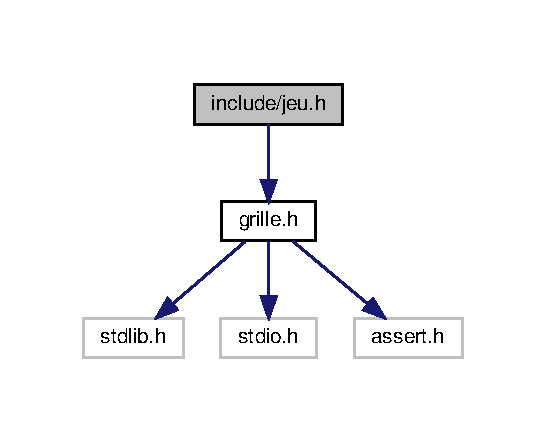
\includegraphics[width=262pt]{jeu_8h__incl}
\end{center}
\end{figure}
This graph shows which files directly or indirectly include this file\+:
\nopagebreak
\begin{figure}[H]
\begin{center}
\leavevmode
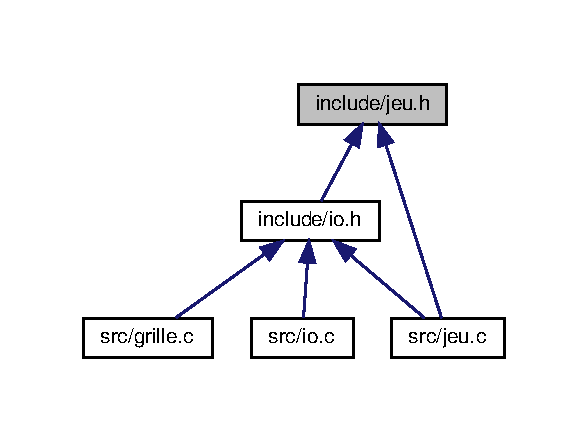
\includegraphics[width=282pt]{jeu_8h__dep__incl}
\end{center}
\end{figure}
\subsection*{Functions}
\begin{DoxyCompactItemize}
\item 
int \hyperlink{jeu_8h_a2e8fdd206d197391527920bbbc137eef}{compte\+\_\+voisins\+\_\+vivants\+\_\+non\+\_\+cyclique} (int i, int j, \hyperlink{structgrille}{grille} g)
\item 
void \hyperlink{jeu_8h_ada8f751a97ad1847db23c5ba17be7802}{evolue} (\hyperlink{structgrille}{grille} $\ast$g, \hyperlink{structgrille}{grille} $\ast$gc)
\item 
int \hyperlink{jeu_8h_a919a35926d94b71717909ecc50233f26}{compte\+\_\+voisins\+\_\+vivants\+\_\+cyclique} (int i, int j, \hyperlink{structgrille}{grille} g)
\end{DoxyCompactItemize}
\subsection*{Variables}
\begin{DoxyCompactItemize}
\item 
\mbox{\Hypertarget{jeu_8h_a56e91f37f1e0eba65fc9f1dd39841b25}\label{jeu_8h_a56e91f37f1e0eba65fc9f1dd39841b25}} 
int($\ast$ {\bfseries voisins\+\_\+vivants} )(int, int, \hyperlink{structgrille}{grille})
\end{DoxyCompactItemize}


\subsection{Detailed Description}
header pour les fonctions d\textquotesingle{}evolution \begin{DoxyAuthor}{Author}
Maxime M\+A\+I\+RE 
\end{DoxyAuthor}


\subsection{Function Documentation}
\mbox{\Hypertarget{jeu_8h_a919a35926d94b71717909ecc50233f26}\label{jeu_8h_a919a35926d94b71717909ecc50233f26}} 
\index{jeu.\+h@{jeu.\+h}!compte\+\_\+voisins\+\_\+vivants\+\_\+cyclique@{compte\+\_\+voisins\+\_\+vivants\+\_\+cyclique}}
\index{compte\+\_\+voisins\+\_\+vivants\+\_\+cyclique@{compte\+\_\+voisins\+\_\+vivants\+\_\+cyclique}!jeu.\+h@{jeu.\+h}}
\subsubsection{\texorpdfstring{compte\+\_\+voisins\+\_\+vivants\+\_\+cyclique()}{compte\_voisins\_vivants\_cyclique()}}
{\footnotesize\ttfamily int compte\+\_\+voisins\+\_\+vivants\+\_\+cyclique (\begin{DoxyParamCaption}\item[{int}]{i,  }\item[{int}]{j,  }\item[{\hyperlink{structgrille}{grille}}]{g }\end{DoxyParamCaption})}


\begin{DoxyParams}{Parameters}
{\em i} & est un entier representant la ieme ligne de la grille g \\
\hline
{\em j} & est un entier representant la jeme colonne de la grille g \\
\hline
{\em g} & est une grille \\
\hline
\end{DoxyParams}
\begin{DoxyReturn}{Returns}
Retourne un entier, representant le nombre de voisin (en mode cyclique) d\textquotesingle{}une case de ligne i et de colonne j d\textquotesingle{}une grille g 
\end{DoxyReturn}
\mbox{\Hypertarget{jeu_8h_a2e8fdd206d197391527920bbbc137eef}\label{jeu_8h_a2e8fdd206d197391527920bbbc137eef}} 
\index{jeu.\+h@{jeu.\+h}!compte\+\_\+voisins\+\_\+vivants\+\_\+non\+\_\+cyclique@{compte\+\_\+voisins\+\_\+vivants\+\_\+non\+\_\+cyclique}}
\index{compte\+\_\+voisins\+\_\+vivants\+\_\+non\+\_\+cyclique@{compte\+\_\+voisins\+\_\+vivants\+\_\+non\+\_\+cyclique}!jeu.\+h@{jeu.\+h}}
\subsubsection{\texorpdfstring{compte\+\_\+voisins\+\_\+vivants\+\_\+non\+\_\+cyclique()}{compte\_voisins\_vivants\_non\_cyclique()}}
{\footnotesize\ttfamily int compte\+\_\+voisins\+\_\+vivants\+\_\+non\+\_\+cyclique (\begin{DoxyParamCaption}\item[{int}]{i,  }\item[{int}]{j,  }\item[{\hyperlink{structgrille}{grille}}]{g }\end{DoxyParamCaption})}


\begin{DoxyParams}{Parameters}
{\em i} & est un entier representant la ieme ligne de la grille g \\
\hline
{\em j} & est un entier representant la jeme colonne de la grille g \\
\hline
{\em g} & est une grille \\
\hline
\end{DoxyParams}
\begin{DoxyReturn}{Returns}
Retourne un entier, representant le nombre de voisin (en mode non cyclique) d\textquotesingle{}une case de ligne i et de colonne j d\textquotesingle{}une grille g 
\end{DoxyReturn}
\mbox{\Hypertarget{jeu_8h_ada8f751a97ad1847db23c5ba17be7802}\label{jeu_8h_ada8f751a97ad1847db23c5ba17be7802}} 
\index{jeu.\+h@{jeu.\+h}!evolue@{evolue}}
\index{evolue@{evolue}!jeu.\+h@{jeu.\+h}}
\subsubsection{\texorpdfstring{evolue()}{evolue()}}
{\footnotesize\ttfamily void evolue (\begin{DoxyParamCaption}\item[{\hyperlink{structgrille}{grille} $\ast$}]{g,  }\item[{\hyperlink{structgrille}{grille} $\ast$}]{gc }\end{DoxyParamCaption})}


\begin{DoxyParams}{Parameters}
{\em $\ast$g} & est un pointeur sur la grille g \\
\hline
{\em $\ast$gc} & est un pointeur sur la grille gc \\
\hline
\end{DoxyParams}
\begin{DoxyReturn}{Returns}
Retourne vide, mais evolue la grille passé en argument 
\end{DoxyReturn}

\hypertarget{grille_8c}{}\section{src/grille.c File Reference}
\label{grille_8c}\index{src/grille.\+c@{src/grille.\+c}}
{\ttfamily \#include \char`\"{}grille.\+h\char`\"{}}\newline
{\ttfamily \#include \char`\"{}io.\+h\char`\"{}}\newline
Include dependency graph for grille.\+c\+:
\nopagebreak
\begin{figure}[H]
\begin{center}
\leavevmode
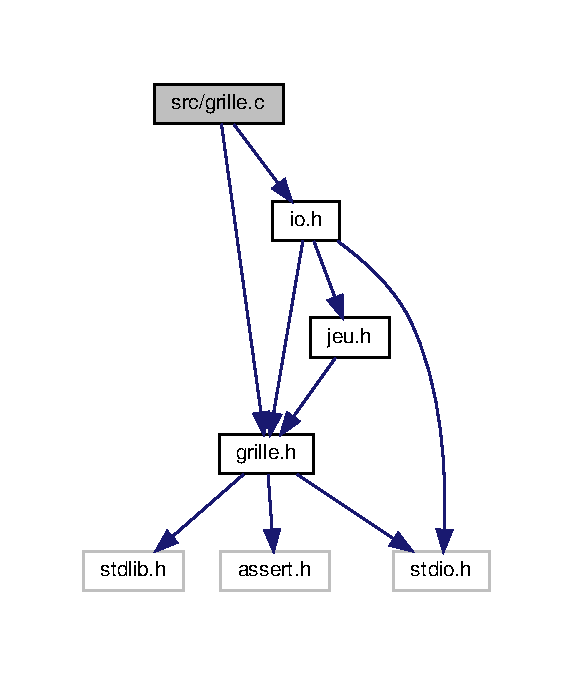
\includegraphics[width=275pt]{grille_8c__incl}
\end{center}
\end{figure}
\subsection*{Functions}
\begin{DoxyCompactItemize}
\item 
void \hyperlink{grille_8c_ae621f51c60aa4fafaa0c9f6c9b5a4036}{alloue\+\_\+grille} (int l, int c, \hyperlink{structgrille}{grille} $\ast$g)
\item 
void \hyperlink{grille_8c_a7074b2b15576e9d2b3cd15c3a1dc7012}{libere\+\_\+grille} (\hyperlink{structgrille}{grille} $\ast$g)
\item 
void \hyperlink{grille_8c_adf5501cc0bbad28f5ffc561d92197e4e}{init\+\_\+grille\+\_\+from\+\_\+file} (char $\ast$filename, \hyperlink{structgrille}{grille} $\ast$g)
\item 
void \hyperlink{grille_8c_a63b3ae16c86b568f6aa8f9ce84128b1e}{copie\+\_\+grille} (\hyperlink{structgrille}{grille} gs, \hyperlink{structgrille}{grille} gd)
\end{DoxyCompactItemize}


\subsection{Detailed Description}
code pour les fonctions sur les grilles \begin{DoxyAuthor}{Author}
Maxime M\+A\+I\+RE 
\end{DoxyAuthor}


\subsection{Function Documentation}
\mbox{\Hypertarget{grille_8c_ae621f51c60aa4fafaa0c9f6c9b5a4036}\label{grille_8c_ae621f51c60aa4fafaa0c9f6c9b5a4036}} 
\index{grille.\+c@{grille.\+c}!alloue\+\_\+grille@{alloue\+\_\+grille}}
\index{alloue\+\_\+grille@{alloue\+\_\+grille}!grille.\+c@{grille.\+c}}
\subsubsection{\texorpdfstring{alloue\+\_\+grille()}{alloue\_grille()}}
{\footnotesize\ttfamily void alloue\+\_\+grille (\begin{DoxyParamCaption}\item[{int}]{l,  }\item[{int}]{c,  }\item[{\hyperlink{structgrille}{grille} $\ast$}]{g }\end{DoxyParamCaption})}


\begin{DoxyParams}{Parameters}
{\em l} & est un entier representant le nombre de ligne a alloue pour la grille g \\
\hline
{\em c} & est un entier representant le nombre de colonne a alloue pour la grille g \\
\hline
{\em $\ast$g} & est un pointeur sur une grille \\
\hline
\end{DoxyParams}
\begin{DoxyReturn}{Returns}
Retourne vide, mais alloue une grille de ligne l et de colonne c 
\end{DoxyReturn}
\mbox{\Hypertarget{grille_8c_a63b3ae16c86b568f6aa8f9ce84128b1e}\label{grille_8c_a63b3ae16c86b568f6aa8f9ce84128b1e}} 
\index{grille.\+c@{grille.\+c}!copie\+\_\+grille@{copie\+\_\+grille}}
\index{copie\+\_\+grille@{copie\+\_\+grille}!grille.\+c@{grille.\+c}}
\subsubsection{\texorpdfstring{copie\+\_\+grille()}{copie\_grille()}}
{\footnotesize\ttfamily void copie\+\_\+grille (\begin{DoxyParamCaption}\item[{\hyperlink{structgrille}{grille}}]{gs,  }\item[{\hyperlink{structgrille}{grille}}]{gd }\end{DoxyParamCaption})}


\begin{DoxyParams}{Parameters}
{\em gs} & est une grille \\
\hline
{\em gd} & est une grille \\
\hline
\end{DoxyParams}
\begin{DoxyReturn}{Returns}
Retourne vide, mais recopie la grille gs dans la grille gd 
\end{DoxyReturn}
\mbox{\Hypertarget{grille_8c_adf5501cc0bbad28f5ffc561d92197e4e}\label{grille_8c_adf5501cc0bbad28f5ffc561d92197e4e}} 
\index{grille.\+c@{grille.\+c}!init\+\_\+grille\+\_\+from\+\_\+file@{init\+\_\+grille\+\_\+from\+\_\+file}}
\index{init\+\_\+grille\+\_\+from\+\_\+file@{init\+\_\+grille\+\_\+from\+\_\+file}!grille.\+c@{grille.\+c}}
\subsubsection{\texorpdfstring{init\+\_\+grille\+\_\+from\+\_\+file()}{init\_grille\_from\_file()}}
{\footnotesize\ttfamily void init\+\_\+grille\+\_\+from\+\_\+file (\begin{DoxyParamCaption}\item[{char $\ast$}]{filename,  }\item[{\hyperlink{structgrille}{grille} $\ast$}]{g }\end{DoxyParamCaption})}


\begin{DoxyParams}{Parameters}
{\em $\ast$filename} & est un tableau de charactere permettant de chercher un fichier a scanf \\
\hline
{\em $\ast$g} & est un pointeur sur une grille \\
\hline
\end{DoxyParams}
\begin{DoxyReturn}{Returns}
Retourne vide, mais alloue et initalise la grille g à partir d\textquotesingle{}un fichier 
\end{DoxyReturn}
\mbox{\Hypertarget{grille_8c_a7074b2b15576e9d2b3cd15c3a1dc7012}\label{grille_8c_a7074b2b15576e9d2b3cd15c3a1dc7012}} 
\index{grille.\+c@{grille.\+c}!libere\+\_\+grille@{libere\+\_\+grille}}
\index{libere\+\_\+grille@{libere\+\_\+grille}!grille.\+c@{grille.\+c}}
\subsubsection{\texorpdfstring{libere\+\_\+grille()}{libere\_grille()}}
{\footnotesize\ttfamily void libere\+\_\+grille (\begin{DoxyParamCaption}\item[{\hyperlink{structgrille}{grille} $\ast$}]{g }\end{DoxyParamCaption})}


\begin{DoxyParams}{Parameters}
{\em $\ast$g} & est un pointeur sur une grille \\
\hline
\end{DoxyParams}
\begin{DoxyReturn}{Returns}
Retourne vide, mais libere la grille g 
\end{DoxyReturn}

\hypertarget{io_8c}{}\section{src/io.c File Reference}
\label{io_8c}\index{src/io.\+c@{src/io.\+c}}
{\ttfamily \#include \char`\"{}io.\+h\char`\"{}}\newline
Include dependency graph for io.\+c\+:\nopagebreak
\begin{figure}[H]
\begin{center}
\leavevmode
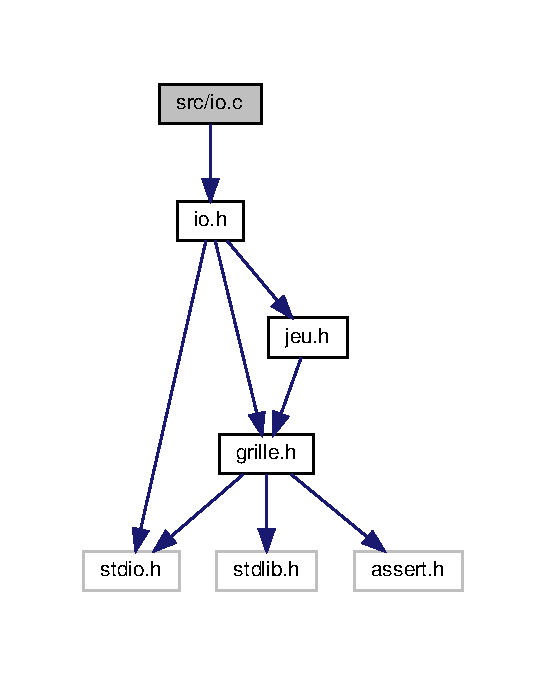
\includegraphics[width=262pt]{io_8c__incl}
\end{center}
\end{figure}
\subsection*{Functions}
\begin{DoxyCompactItemize}
\item 
void \hyperlink{io_8c_a634cf584c380ce221d5d4199f3e813bd}{affiche\+\_\+trait} (int c)
\item 
void \hyperlink{io_8c_a3f3ff78e56fcf21a932ff73b70635554}{affiche\+\_\+ligne} (int c, int $\ast$ligne)
\item 
void \hyperlink{io_8c_a90cb8ec05374b46d9995705ed4954f34}{affiche\+\_\+grille} (\hyperlink{structgrille}{grille} g)
\item 
void \hyperlink{io_8c_ab36a6f8957cd3e682119007836ce6ad5}{efface\+\_\+grille} (\hyperlink{structgrille}{grille} g)
\item 
void \hyperlink{io_8c_a88493b3c55828670e47150a95ed7db5b}{debut\+\_\+jeu} (\hyperlink{structgrille}{grille} $\ast$g, \hyperlink{structgrille}{grille} $\ast$gc)
\end{DoxyCompactItemize}


\subsection{Detailed Description}
code pour les fonctions d\textquotesingle{}affichages \begin{DoxyAuthor}{Author}
Maxime M\+A\+I\+RE 
\end{DoxyAuthor}


\subsection{Function Documentation}
\mbox{\Hypertarget{io_8c_a90cb8ec05374b46d9995705ed4954f34}\label{io_8c_a90cb8ec05374b46d9995705ed4954f34}} 
\index{io.\+c@{io.\+c}!affiche\+\_\+grille@{affiche\+\_\+grille}}
\index{affiche\+\_\+grille@{affiche\+\_\+grille}!io.\+c@{io.\+c}}
\subsubsection{\texorpdfstring{affiche\+\_\+grille()}{affiche\_grille()}}
{\footnotesize\ttfamily void affiche\+\_\+grille (\begin{DoxyParamCaption}\item[{\hyperlink{structgrille}{grille}}]{g }\end{DoxyParamCaption})}


\begin{DoxyParams}{Parameters}
{\em g} & est une grille \\
\hline
\end{DoxyParams}
\begin{DoxyReturn}{Returns}
Retourne vide, mais affiche la grille g 
\end{DoxyReturn}
\mbox{\Hypertarget{io_8c_a3f3ff78e56fcf21a932ff73b70635554}\label{io_8c_a3f3ff78e56fcf21a932ff73b70635554}} 
\index{io.\+c@{io.\+c}!affiche\+\_\+ligne@{affiche\+\_\+ligne}}
\index{affiche\+\_\+ligne@{affiche\+\_\+ligne}!io.\+c@{io.\+c}}
\subsubsection{\texorpdfstring{affiche\+\_\+ligne()}{affiche\_ligne()}}
{\footnotesize\ttfamily void affiche\+\_\+ligne (\begin{DoxyParamCaption}\item[{int}]{c,  }\item[{int $\ast$}]{ligne }\end{DoxyParamCaption})}


\begin{DoxyParams}{Parameters}
{\em c} & est le nombre de colonne a affiché \\
\hline
{\em ligne} & est un pointeur sur entier \\
\hline
\end{DoxyParams}
\begin{DoxyReturn}{Returns}
Retourne vide, mais affiche des caracteres 
\end{DoxyReturn}
\mbox{\Hypertarget{io_8c_a634cf584c380ce221d5d4199f3e813bd}\label{io_8c_a634cf584c380ce221d5d4199f3e813bd}} 
\index{io.\+c@{io.\+c}!affiche\+\_\+trait@{affiche\+\_\+trait}}
\index{affiche\+\_\+trait@{affiche\+\_\+trait}!io.\+c@{io.\+c}}
\subsubsection{\texorpdfstring{affiche\+\_\+trait()}{affiche\_trait()}}
{\footnotesize\ttfamily void affiche\+\_\+trait (\begin{DoxyParamCaption}\item[{int}]{c }\end{DoxyParamCaption})}


\begin{DoxyParams}{Parameters}
{\em c} & est le nombre de colonne a affiché \\
\hline
\end{DoxyParams}
\begin{DoxyReturn}{Returns}
Retourne vide, mais affiche des caracteres 
\end{DoxyReturn}
\mbox{\Hypertarget{io_8c_a88493b3c55828670e47150a95ed7db5b}\label{io_8c_a88493b3c55828670e47150a95ed7db5b}} 
\index{io.\+c@{io.\+c}!debut\+\_\+jeu@{debut\+\_\+jeu}}
\index{debut\+\_\+jeu@{debut\+\_\+jeu}!io.\+c@{io.\+c}}
\subsubsection{\texorpdfstring{debut\+\_\+jeu()}{debut\_jeu()}}
{\footnotesize\ttfamily void debut\+\_\+jeu (\begin{DoxyParamCaption}\item[{\hyperlink{structgrille}{grille} $\ast$}]{g,  }\item[{\hyperlink{structgrille}{grille} $\ast$}]{gc }\end{DoxyParamCaption})}


\begin{DoxyParams}{Parameters}
{\em $\ast$g} & est un pointeur sur la grille g \\
\hline
{\em $\ast$gc} & est un pointeur sur la grille gc \\
\hline
\end{DoxyParams}
\begin{DoxyReturn}{Returns}
Retourne vide, mais efface la grille g 
\end{DoxyReturn}
\mbox{\Hypertarget{io_8c_ab36a6f8957cd3e682119007836ce6ad5}\label{io_8c_ab36a6f8957cd3e682119007836ce6ad5}} 
\index{io.\+c@{io.\+c}!efface\+\_\+grille@{efface\+\_\+grille}}
\index{efface\+\_\+grille@{efface\+\_\+grille}!io.\+c@{io.\+c}}
\subsubsection{\texorpdfstring{efface\+\_\+grille()}{efface\_grille()}}
{\footnotesize\ttfamily void efface\+\_\+grille (\begin{DoxyParamCaption}\item[{\hyperlink{structgrille}{grille}}]{g }\end{DoxyParamCaption})}


\begin{DoxyParams}{Parameters}
{\em g} & est une grille \\
\hline
\end{DoxyParams}
\begin{DoxyReturn}{Returns}
Retourne vide, mais efface la grille g 
\end{DoxyReturn}

\hypertarget{jeu_8c}{}\section{src/jeu.c File Reference}
\label{jeu_8c}\index{src/jeu.\+c@{src/jeu.\+c}}
{\ttfamily \#include \char`\"{}jeu.\+h\char`\"{}}\newline
{\ttfamily \#include \char`\"{}io.\+h\char`\"{}}\newline
{\ttfamily \#include \char`\"{}grille.\+h\char`\"{}}\newline
Include dependency graph for jeu.\+c\+:
\nopagebreak
\begin{figure}[H]
\begin{center}
\leavevmode
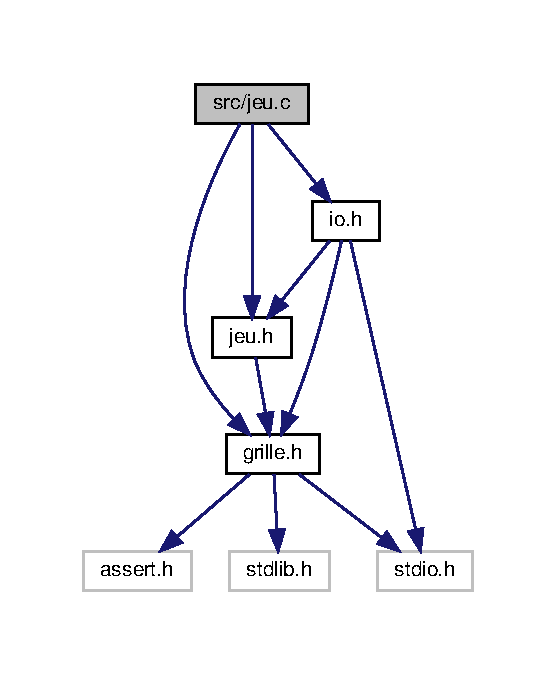
\includegraphics[width=267pt]{jeu_8c__incl}
\end{center}
\end{figure}
\subsection*{Functions}
\begin{DoxyCompactItemize}
\item 
int \hyperlink{jeu_8c_a919a35926d94b71717909ecc50233f26}{compte\+\_\+voisins\+\_\+vivants\+\_\+cyclique} (int i, int j, \hyperlink{structgrille}{grille} g)
\item 
int \hyperlink{jeu_8c_a2e8fdd206d197391527920bbbc137eef}{compte\+\_\+voisins\+\_\+vivants\+\_\+non\+\_\+cyclique} (int i, int j, \hyperlink{structgrille}{grille} g)
\item 
void \hyperlink{jeu_8c_ada8f751a97ad1847db23c5ba17be7802}{evolue} (\hyperlink{structgrille}{grille} $\ast$g, \hyperlink{structgrille}{grille} $\ast$gc)
\end{DoxyCompactItemize}


\subsection{Detailed Description}
code pour les fonctions d\textquotesingle{}evolutions \begin{DoxyAuthor}{Author}
Maxime M\+A\+I\+RE 
\end{DoxyAuthor}


\subsection{Function Documentation}
\mbox{\Hypertarget{jeu_8c_a919a35926d94b71717909ecc50233f26}\label{jeu_8c_a919a35926d94b71717909ecc50233f26}} 
\index{jeu.\+c@{jeu.\+c}!compte\+\_\+voisins\+\_\+vivants\+\_\+cyclique@{compte\+\_\+voisins\+\_\+vivants\+\_\+cyclique}}
\index{compte\+\_\+voisins\+\_\+vivants\+\_\+cyclique@{compte\+\_\+voisins\+\_\+vivants\+\_\+cyclique}!jeu.\+c@{jeu.\+c}}
\subsubsection{\texorpdfstring{compte\+\_\+voisins\+\_\+vivants\+\_\+cyclique()}{compte\_voisins\_vivants\_cyclique()}}
{\footnotesize\ttfamily int compte\+\_\+voisins\+\_\+vivants\+\_\+cyclique (\begin{DoxyParamCaption}\item[{int}]{i,  }\item[{int}]{j,  }\item[{\hyperlink{structgrille}{grille}}]{g }\end{DoxyParamCaption})}


\begin{DoxyParams}{Parameters}
{\em i} & est un entier representant la ieme ligne de la grille g \\
\hline
{\em j} & est un entier representant la jeme colonne de la grille g \\
\hline
{\em g} & est une grille \\
\hline
\end{DoxyParams}
\begin{DoxyReturn}{Returns}
Retourne un entier, representant le nombre de voisin (en mode cyclique) d\textquotesingle{}une case de ligne i et de colonne j d\textquotesingle{}une grille g 
\end{DoxyReturn}
\mbox{\Hypertarget{jeu_8c_a2e8fdd206d197391527920bbbc137eef}\label{jeu_8c_a2e8fdd206d197391527920bbbc137eef}} 
\index{jeu.\+c@{jeu.\+c}!compte\+\_\+voisins\+\_\+vivants\+\_\+non\+\_\+cyclique@{compte\+\_\+voisins\+\_\+vivants\+\_\+non\+\_\+cyclique}}
\index{compte\+\_\+voisins\+\_\+vivants\+\_\+non\+\_\+cyclique@{compte\+\_\+voisins\+\_\+vivants\+\_\+non\+\_\+cyclique}!jeu.\+c@{jeu.\+c}}
\subsubsection{\texorpdfstring{compte\+\_\+voisins\+\_\+vivants\+\_\+non\+\_\+cyclique()}{compte\_voisins\_vivants\_non\_cyclique()}}
{\footnotesize\ttfamily int compte\+\_\+voisins\+\_\+vivants\+\_\+non\+\_\+cyclique (\begin{DoxyParamCaption}\item[{int}]{i,  }\item[{int}]{j,  }\item[{\hyperlink{structgrille}{grille}}]{g }\end{DoxyParamCaption})}


\begin{DoxyParams}{Parameters}
{\em i} & est un entier representant la ieme ligne de la grille g \\
\hline
{\em j} & est un entier representant la jeme colonne de la grille g \\
\hline
{\em g} & est une grille \\
\hline
\end{DoxyParams}
\begin{DoxyReturn}{Returns}
Retourne un entier, representant le nombre de voisin (en mode non cyclique) d\textquotesingle{}une case de ligne i et de colonne j d\textquotesingle{}une grille g 
\end{DoxyReturn}
\mbox{\Hypertarget{jeu_8c_ada8f751a97ad1847db23c5ba17be7802}\label{jeu_8c_ada8f751a97ad1847db23c5ba17be7802}} 
\index{jeu.\+c@{jeu.\+c}!evolue@{evolue}}
\index{evolue@{evolue}!jeu.\+c@{jeu.\+c}}
\subsubsection{\texorpdfstring{evolue()}{evolue()}}
{\footnotesize\ttfamily void evolue (\begin{DoxyParamCaption}\item[{\hyperlink{structgrille}{grille} $\ast$}]{g,  }\item[{\hyperlink{structgrille}{grille} $\ast$}]{gc }\end{DoxyParamCaption})}


\begin{DoxyParams}{Parameters}
{\em $\ast$g} & est un pointeur sur la grille g \\
\hline
{\em $\ast$gc} & est un pointeur sur la grille gc \\
\hline
\end{DoxyParams}
\begin{DoxyReturn}{Returns}
Retourne vide, mais evolue la grille passé en argument 
\end{DoxyReturn}

%--- End generated contents ---

% Index
\backmatter
\newpage
\phantomsection
\clearemptydoublepage
\addcontentsline{toc}{chapter}{Index}
\printindex

\end{document}
